\batchmode
\makeatletter
\def\input@path{{/Users/sergei.winitzki/Code/talks/join_calculus/}}
\makeatother
\documentclass[english]{beamer}
\usepackage[T1]{fontenc}
\usepackage[latin9]{inputenc}
\setcounter{secnumdepth}{3}
\setcounter{tocdepth}{3}
\usepackage{babel}
\usepackage{array}
\usepackage{calc}
\usepackage{amstext}
\usepackage{graphicx}
\ifx\hypersetup\undefined
  \AtBeginDocument{%
    \hypersetup{unicode=true,pdfusetitle,
 bookmarks=true,bookmarksnumbered=false,bookmarksopen=false,
 breaklinks=false,pdfborder={0 0 1},backref=false,colorlinks=true}
  }
\else
  \hypersetup{unicode=true,pdfusetitle,
 bookmarks=true,bookmarksnumbered=false,bookmarksopen=false,
 breaklinks=false,pdfborder={0 0 1},backref=false,colorlinks=true}
\fi

\makeatletter

%%%%%%%%%%%%%%%%%%%%%%%%%%%%%% LyX specific LaTeX commands.
%% Because html converters don't know tabularnewline
\providecommand{\tabularnewline}{\\}

%%%%%%%%%%%%%%%%%%%%%%%%%%%%%% Textclass specific LaTeX commands.
% this default might be overridden by plain title style
\newcommand\makebeamertitle{\frame{\maketitle}}%
% (ERT) argument for the TOC
\AtBeginDocument{%
  \let\origtableofcontents=\tableofcontents
  \def\tableofcontents{\@ifnextchar[{\origtableofcontents}{\gobbletableofcontents}}
  \def\gobbletableofcontents#1{\origtableofcontents}
}
\newenvironment{lyxcode}
  {\par\begin{list}{}{
    \setlength{\rightmargin}{\leftmargin}
    \setlength{\listparindent}{0pt}% needed for AMS classes
    \raggedright
    \setlength{\itemsep}{0pt}
    \setlength{\parsep}{0pt}
    \normalfont\ttfamily}%
   \def\{{\char`\{}
   \def\}{\char`\}}
   \def\textasciitilde{\char`\~}
   \item[]}
  {\end{list}}

%%%%%%%%%%%%%%%%%%%%%%%%%%%%%% User specified LaTeX commands.
\usetheme[secheader]{Boadilla}
\usecolortheme{seahorse}
\author{Sergei Winitzki}
\date{November 16, 2018}
\setbeamertemplate{headline}{} % disable headline at top
\setbeamertemplate{navigation symbols}{} % disable navigation bar at bottom
\title[Declarative distributed concurrency]{Declarative distributed concurrency in Scala}
\institute[SBTB 2018]{Scale by the Bay 2018}

\makeatother

\begin{document}
\frame{\titlepage}
\begin{frame}{Talk summary}


\framesubtitle{How I learned to forget semaphores and to love concurrency}

\texttt{Chymyst} = an implementation of the Chemical Machine (CM)
paradigm
\begin{itemize}
\item CM $\approx$ Actors made purely functional and auto-parallelized
\item Intuitions about why CM works better than other concurrency models
\begin{itemize}
\item Comparison with related work: ING Baker, BPMN (workflow)
\end{itemize}
\item New extension for distributed programming: DCM
\item Code examples
\end{itemize}
Not in this talk: academic theory
\begin{itemize}
\item Petri nets, $\pi$-calculus, join calculus, joinads, mobile agent
calculus...
\item DCM formulated within a theory of distributed programming?
\end{itemize}
\end{frame}

\begin{frame}{Concurrent \& parallel programming: How we cope}

\emph{Imperative} concurrency \& parallelism is difficult to reason
about:
\begin{itemize}
\item low-level API: callbacks, threads, semaphores, mutex locks
\item hard to reason about mutable state and running processes
\item hard to test -- non-deterministic runtime behavior!
\begin{itemize}
\item race conditions, deadlocks, livelocks
\end{itemize}
\end{itemize}
\begin{center}
\vspace{-0.2cm}
Known declarative approaches to avoid these problems:\vspace{-0.5cm}
\par\end{center}

\begin{center}
\begin{tabular}{|>{\centering}p{0.35\textwidth}|c|>{\centering}p{0.3\textwidth}|}
\hline 
\textbf{\footnotesize{}Kind of concurrency} &
\textbf{\footnotesize{}Typeclass} &
\textbf{\footnotesize{}Scala implementation}\tabularnewline
\hline 
\hline 
synchronous parallelism &
applicative functor &
Spark, \texttt{\textcolor{blue}{\scriptsize{}.par.map()}}\tabularnewline
\hline 
asynchronous streaming DAG &
monadic functor &
\texttt{\textcolor{blue}{\scriptsize{}Future}}, \texttt{\textcolor{blue}{\scriptsize{}async}}{\footnotesize{}/}\texttt{\textcolor{blue}{\scriptsize{}await}},
\texttt{\footnotesize{}RxJava}, Akka Streams\tabularnewline
\hline 
unrestricted streaming &
recursive monad+ &
Flink, fs2, ZIO\tabularnewline
\hline 
unrestricted concurrency &
? &
Akka, \texttt{\footnotesize{}Chymyst}\tabularnewline
\hline 
\end{tabular}
\par\end{center}

For distributed computing: challenges remain
\begin{itemize}
\item coordination and consensus, persistence and fault tolerance
\item cluster configuration and discovery
\begin{itemize}
\item distributed coordination as a service: Apache ZooKeeper, \texttt{etcd}
\end{itemize}
\end{itemize}
\end{frame}

\begin{frame}{``Dining philosophers''}


\framesubtitle{The paradigmatic example of concurrency, parallelism and resource
contention}

\href{https://en.wikipedia.org/wiki/Dining_philosophers_problem}{Five philosophers sit at a round table},
taking turns eating and thinking for random time intervals
\begin{center}
\includegraphics[height=4cm]{3_Users_sergei_win\includegraphics[height=4cm]{An_illustration_of_the_dining_philosophers_problem}
\par\end{center}

Problem: simulate the process, avoiding deadlock and starvation

Solutions in various programming languages: see \href{https://rosettacode.org/wiki/Dining_philosophers}{Rosetta Code}
\begin{itemize}
\item Can this be implemented via (effectful) streams?
\begin{itemize}
\item (I think not: a stream expression can be run on a single CPU thread.)
\end{itemize}
\item The Chemical Machine code is purely declarative
\end{itemize}
\end{frame}

\begin{frame}{What is the Chemical Machine}

The Chemical Machine paradigm:
\begin{itemize}
\item A \emph{declarative language} for concurrent and parallel computations
\begin{itemize}
\item largely unknown and unused by the software engineering community
\item \texttt{Chymyst} -- an \href{https://github.com/Chymyst/chymyst-core}{open-source library \& embedded DSL}
for Scala
\item presented in my SBTB talks in 2016 and 2017
\end{itemize}
\item Implement anything in 10-15 lines of code
\item Derive programs quickly from specifications
\end{itemize}
\end{frame}

\begin{frame}{Chemical Machine vs.~Amazon's AWS Lambda}

How AWS$\lambda$ works:
\begin{itemize}
\item wait for an event that signals arrival of input data
\item run a computation whenever input data becomes available
\item the computation is automatically parallelized, data-driven
\item writing the output data will create a new event
\end{itemize}
Modify the AWS$\lambda$ execution model by adding new requirements:
\begin{itemize}
\item a Lambda should be able to wait for several \emph{unrelated} events
\item several Lambdas may contend \emph{atomically} on shared input events
\end{itemize}
With these new requirements, AWS$\lambda$ becomes ``AWS$\pi$''
-- a model of ``unrestricted concurrency''
\begin{itemize}
\item (Implementation on AWS will be tricky)
\end{itemize}
\end{frame}

\begin{frame}{The Chemical Machine vs.~the Actor model}

Modify the Actor execution model by adding new requirements:
\begin{itemize}
\item when messages arrive, actors are auto-created, maybe \emph{in parallel}
\item actors may wait atomically for messages in \emph{several} different
mailboxes
\end{itemize}
It follows from these requirements that... 
\begin{itemize}
\item Auto-created actor instances are \emph{stateless} and invisible to
user
\item User code defines \emph{mailboxes} and \emph{computations} that consume
messages
\item Repeated messages may be consumed in parallel
\item Messages are sent to mailboxes, not to specific actor instances:
\end{itemize}
\begin{minipage}[c][1\totalheight][t]{0.5\columnwidth}%
\begin{lyxcode}
\textcolor{blue}{\scriptsize{}//~Akka}{\scriptsize\par}

\textcolor{blue}{\scriptsize{}val~a:~ActorRef~=~...~receive(x)~$\Rightarrow$...}{\scriptsize\par}

\textcolor{blue}{\scriptsize{}val~b:~ActorRef~=~...~receive(y)~$\Rightarrow$...}{\scriptsize\par}

\textcolor{blue}{\scriptsize{}a~!~100}{\scriptsize\par}

\textcolor{blue}{\scriptsize{}b~!~1;~~~b~!~2;~~~b~!~3}{\scriptsize\par}
\end{lyxcode}
%
\end{minipage}\hfill{}%
\begin{minipage}[c][1\totalheight][t]{0.45\columnwidth}%
\begin{lyxcode}
\textcolor{blue}{\scriptsize{}//~Chymyst}{\scriptsize\par}

\textcolor{blue}{\scriptsize{}...~go~\{~case~a(x)~$\Rightarrow$~...~\}~}{\scriptsize\par}

\textcolor{blue}{\scriptsize{}...~go~\{~case~b(y)~+~c(z)~$\Rightarrow$~...~\}}{\scriptsize\par}

\textcolor{blue}{\scriptsize{}a(100)}{\scriptsize\par}

\textcolor{blue}{\scriptsize{}b(1);~~b(2);~~b(3);~c(\textquotedbl hello\textquotedbl );}{\scriptsize\par}
\end{lyxcode}
%
\end{minipage}\hfill{}
\begin{itemize}
\item All data resides on messages in mailboxes, is consumed automatically
\item Mailboxes and computations are \emph{values}, can be sent on messages
\end{itemize}
Any Actor program can be straightforwardly translated into CM
\end{frame}

\begin{frame}{Understanding the CM via the chemical metaphor}


\framesubtitle{From real to abstract chemistry}

Real chemistry is ``asynchronous'', ``concurrent'', and ``distributed''
\[
\text{HCl}+\text{NaOH}\rightarrow\text{NaCl}+\text{H}_{2}\text{O}
\]

Want to run \emph{computations} similarly to how chemical reactions
run!

Begin by formulating the execution model of ``abstract chemistry'':
\begin{itemize}
\item Abstract ``molecules'' float around in a ``chemical reaction site''
\item Certain sorts of molecules may combine to start a ``reaction'':
\end{itemize}
~\\

\fbox{\begin{minipage}[c][1\totalheight][t]{0.5\columnwidth}%
\begin{center}
Abstract chemical laws:\\
\texttt{\textcolor{blue}{\footnotesize{}a + b ${\color{blue}\rightarrow}$
a}}\\
\texttt{\textcolor{blue}{\footnotesize{}a + c ${\color{blue}\rightarrow}$
$\textrm{�}$}}
\par\end{center}%
\end{minipage}}\hfill{}%
\begin{minipage}[c][1\totalheight][t]{0.3\columnwidth}%
\includegraphics[width=1\columnwidth]{cham1a}%
\end{minipage}\hfill{}

~\\

\begin{itemize}
\item Program code defines molecules \texttt{\textcolor{blue}{\scriptsize{}a}},
\texttt{\textcolor{blue}{\scriptsize{}b}}, \texttt{\textcolor{blue}{\scriptsize{}c}},
... and chemical laws
\item At initial time, the code emits some molecules into the site
\item The runtime system evolves the molecules \emph{in parallel}
\begin{itemize}
\item A simulator for this is easy to implement in any language
\end{itemize}
\end{itemize}
\end{frame}

\begin{frame}{Chemical Machine in a nutshell}


\framesubtitle{From abstract chemistry to computation}

Translating the chemical metaphor into a model of computation:~\\
~

\fbox{\begin{minipage}[c][1\totalheight][t]{0.5\columnwidth}%
\begin{itemize}
\item Each molecule carries a \textbf{value} (``concurrent data'')
\item Each reaction computes new values from its input values
\item Some molecules with new values may be emitted back into the reaction
site
\end{itemize}
%
\end{minipage}}\hfill{}%
\begin{minipage}[c][1\totalheight][t]{0.45\columnwidth}%
\includegraphics[width=1\columnwidth]{cham2}

~\\
\texttt{\textcolor{blue}{\scriptsize{}site(}}{\scriptsize\par}

\texttt{\textcolor{blue}{\scriptsize{}~ go \{ case }}\texttt{\textbf{\textcolor{blue}{\scriptsize{}a}}}\texttt{\textcolor{blue}{\scriptsize{}(x)
+ }}\texttt{\textbf{\textcolor{blue}{\scriptsize{}b}}}\texttt{\textcolor{blue}{\scriptsize{}(y)
$\Rightarrow$}}{\scriptsize\par}

\texttt{\textcolor{blue}{\scriptsize{}~ ~val z = f(x, y); }}\texttt{\textbf{\textcolor{blue}{\scriptsize{}a}}}\texttt{\textcolor{blue}{\scriptsize{}(z)
\},}}{\scriptsize\par}

\texttt{\textcolor{blue}{\scriptsize{}~ go \{ case }}\texttt{\textbf{\textcolor{blue}{\scriptsize{}a}}}\texttt{\textcolor{blue}{\scriptsize{}(x)
+ }}\texttt{\textbf{\textcolor{blue}{\scriptsize{}c}}}\texttt{\textcolor{blue}{\scriptsize{}(\_)
$\Rightarrow$}}{\scriptsize\par}

\texttt{\textcolor{blue}{\scriptsize{}~ ~ ~ println(x) \}}}{\scriptsize\par}

\texttt{\textcolor{blue}{\scriptsize{})}}{\scriptsize\par}%
\end{minipage}\hfill{}\\
~\\
When a reaction starts: input molecules disappear, new values are
computed, output molecules are emitted

Reactions are \emph{functions} from input values to output values
\begin{itemize}
\item Need to learn how to ``think in molecules''
\end{itemize}
\end{frame}

\begin{frame}{Chemical Machine vs.~Actor model}

\begin{itemize}
\item \vspace{-0.3cm}
reaction $\approx$ function body for an (auto-started) actor
\item emitted molecule with value $\approx$ message with value, in a mailbox
\item molecule emitters $\approx$ mailbox references
\end{itemize}
Programming with actors: 
\begin{itemize}
\item user code creates and manages explicit actor instances
\item actors typically hold mutable state and/or mutate ``behavior''
\begin{itemize}
\item reasoning is about running processes \emph{and} the data sent on messages
\end{itemize}
\end{itemize}
Programming with the Chemical Machine:
\begin{itemize}
\item processes auto-start when the needed input molecules are available
\item many reactions may start at once, with automatic parallelism
\begin{itemize}
\item user code does not manipulate references to processes
\begin{itemize}
\item no state, no supervision, no lifecycle, no ``dead letters'', no
routers
\end{itemize}
\item reasoning is only about the \emph{data} \emph{currently} \emph{available}
on molecules
\begin{itemize}
\item no reasoning about running processes having state
\end{itemize}
\end{itemize}
\end{itemize}
\texttt{Chymyst} code is typically 2x -- 3x shorter than equivalent
Akka code
\end{frame}

\begin{frame}{Example: throttling}

Throttle emitting molecules \texttt{\textcolor{blue}{\footnotesize{}s(x)}}
with minimum allowed delay of \texttt{\textcolor{blue}{\footnotesize{}delta}}
ms
\begin{lyxcode}
\textcolor{blue}{\footnotesize{}def~throttle{[}X{]}(s:~M{[}X{]},~delta:~Long):~M{[}X{]}~=~\{}{\footnotesize\par}

\textcolor{blue}{\footnotesize{}~val~r~=~m{[}X{]}}{\footnotesize\par}

\textcolor{blue}{\footnotesize{}~val~enable~=~m{[}Unit{]}~}\textcolor{gray}{\scriptsize{}//~This~molecule~is~confined~to~the~local~scope.}{\scriptsize\par}

\textcolor{blue}{\footnotesize{}~site(}{\footnotesize\par}

\textcolor{blue}{\footnotesize{}~~go~\{~case~r(x)~+~enable(\_)~\ensuremath{\Rightarrow}}{\footnotesize\par}

\textcolor{blue}{\footnotesize{}~~~~~~~~s(x)}{\footnotesize\par}

\textcolor{blue}{\footnotesize{}~~~~~~~~Thread.sleep(delta)}{\footnotesize\par}

\textcolor{blue}{\footnotesize{}~~~~~~~~enable()}{\footnotesize\par}

\textcolor{blue}{\footnotesize{}~~~~~\}}{\footnotesize\par}

\textcolor{blue}{\footnotesize{}~)}{\footnotesize\par}

\textcolor{blue}{\footnotesize{}~enable()~}\textcolor{gray}{\scriptsize{}//~Enable~emitting~`s`~initially.}{\scriptsize\par}

\textcolor{blue}{\footnotesize{}~r~}\textcolor{gray}{\scriptsize{}//~Outside~scope~will~be~able~to~emit~`r`.}{\scriptsize\par}

\textcolor{blue}{\footnotesize{}\}}{\footnotesize\par}
\end{lyxcode}
\begin{itemize}
\item No threads/semaphores/locks, no mutable state
\item External code may emit \texttt{\textcolor{blue}{\footnotesize{}r(x)}}
at will, and \texttt{\textcolor{blue}{\footnotesize{}s(x)}} is then
throttled
\end{itemize}
\href{ https://github.com/softwaremill/akka-vs-scalaz/tree/master/core/src/main/scala/com/softwaremill/ratelimiter}{Implementations in Akka, in Monix, and ZIO}:
> 50 LOC each
\end{frame}

\begin{frame}{Example: map/reduce}

A simple map/reduce implementation:
\begin{lyxcode}
\textcolor{blue}{\scriptsize{}val~c~=~m{[}A{]}}\textcolor{gray}{\scriptsize{}~//~Initial~values~have~type~`A`.}{\scriptsize\par}

\textcolor{blue}{\scriptsize{}val~d~=~m{[}(Int,~B){]}~}\textcolor{gray}{\scriptsize{}//~`B`~is~a~commutative~monoid.}{\scriptsize\par}

\textcolor{blue}{\scriptsize{}val~res~=~m{[}B{]}}\textcolor{gray}{\scriptsize{}~//~Final~result~of~type~`B`.}{\scriptsize\par}

\textcolor{blue}{\scriptsize{}val~fetch~=~b{[}Unit,~B{]}}\textcolor{gray}{\scriptsize{}~//~Blocking~emitter.}{\scriptsize\par}

\textcolor{blue}{\scriptsize{}site(}{\scriptsize\par}

\textcolor{gray}{\scriptsize{}~~//~``map''}{\scriptsize\par}

\textcolor{blue}{\scriptsize{}~~go~\{~case~c(x)~$\Rightarrow$~d((1,~long\_computation(x)))~\},~}{\scriptsize\par}

\textcolor{blue}{\scriptsize{}~}\textcolor{gray}{\scriptsize{}~//~``reduce''}{\scriptsize\par}

\textcolor{blue}{\scriptsize{}~~go~\{~case~d((n1,~b1))~+~d((n2,~b2))~$\Rightarrow$}{\scriptsize\par}

\textcolor{blue}{\scriptsize{}~~~val~(newN,~newB)~=~(n1~+~n2,~b1~|+|~b2)}{\scriptsize\par}

\textcolor{blue}{\scriptsize{}~~~if~(newN~==~total)~res(newB)~else~d((newN,~newB))~}{\scriptsize\par}

\textcolor{blue}{\scriptsize{}~~\},}{\scriptsize\par}

\textcolor{blue}{\scriptsize{}~~go~\{~case~fetch(\_,~reply)~+~res(b)~$\Rightarrow$~reply(b)~\}}{\scriptsize\par}

\textcolor{blue}{\scriptsize{})}{\scriptsize\par}

\textcolor{blue}{\scriptsize{}(1~to~100).foreach(x~$\Rightarrow$~c(x))}{\scriptsize\par}

\textcolor{blue}{\scriptsize{}fetch()}\textcolor{gray}{\footnotesize{}~}\textcolor{gray}{\scriptsize{}//~Blocking~call~will~return~the~final~result.}{\scriptsize\par}
\end{lyxcode}
~\\
Compare with the \href{https://stackoverflow.com/questions/17291851/mapreduce-implementation-with-akka}{Akka implementation here}
(100+ LOC)
\end{frame}

\begin{frame}{Example: parallel merge-sort}

\texttt{Chymyst} code: \href{https://github.com/Chymyst/jc-talk-2017-examples/blob/master/src/test/scala/io/chymyst/talk_examples/MergeSortSpec.scala}{MergeSortSpec.scala}
\begin{lyxcode}
\textcolor{blue}{\scriptsize{}val~mergesort~=~m{[}(Array{[}T{]},~M{[}Array{[}T{]}{]}){]}}{\scriptsize\par}

\textcolor{blue}{\scriptsize{}site(}{\scriptsize\par}

\textcolor{blue}{\scriptsize{}~~go~\{~case~mergesort((arr,~}\textcolor{brown}{\scriptsize{}sortedResult}\textcolor{blue}{\scriptsize{}))~$\Rightarrow$}{\scriptsize\par}

\textcolor{blue}{\scriptsize{}~~~~if~(arr.length~<=~1)~sortedResult(arr)}{\scriptsize\par}

\textcolor{blue}{\scriptsize{}~~~~~~else~\{}{\scriptsize\par}

\textcolor{blue}{\scriptsize{}~~~~~~~~val~}\textcolor{brown}{\scriptsize{}sorted1}\textcolor{blue}{\scriptsize{}~=~m{[}Array{[}T{]}{]}}{\scriptsize\par}

\textcolor{blue}{\scriptsize{}~~~~~~~~val~}\textcolor{brown}{\scriptsize{}sorted2}\textcolor{blue}{\scriptsize{}~=~m{[}Array{[}T{]}{]}}{\scriptsize\par}

\textcolor{blue}{\scriptsize{}~~~~~~~~}\textcolor{brown}{\scriptsize{}site}\textcolor{blue}{\scriptsize{}(}{\scriptsize\par}

\textcolor{blue}{\scriptsize{}~~~~~~~~~~go~\{~case~}\textcolor{brown}{\scriptsize{}sorted1}\textcolor{blue}{\scriptsize{}(x)~+~}\textcolor{brown}{\scriptsize{}sorted2}\textcolor{blue}{\scriptsize{}(y)~$\Rightarrow$}{\scriptsize\par}

\textcolor{brown}{\scriptsize{}~~~~~~~~~~~~~sortedResult}\textcolor{blue}{\scriptsize{}(arrayMerge(x,y))}{\scriptsize\par}

\textcolor{blue}{\scriptsize{}~~~~~~~~~~~~~\}}{\scriptsize\par}

\textcolor{blue}{\scriptsize{}~~~~~~~~)}{\scriptsize\par}

\textcolor{blue}{\scriptsize{}~~~~~~~~val~(part1,~part2)~=~arr.splitAt(arr.length/2)}{\scriptsize\par}

\textcolor{blue}{\scriptsize{}~~~~~~~~}\textsf{\textcolor{gray}{\footnotesize{}//~Emit~lower-level~}}\textcolor{gray}{\footnotesize{}mergesort}\textsf{\textcolor{gray}{\footnotesize{}~molecules:}}{\footnotesize\par}

\textcolor{blue}{\scriptsize{}~~~~~~~~mergesort(part1,~}\textcolor{brown}{\scriptsize{}sorted1}\textcolor{blue}{\scriptsize{})~+~mergesort(part2,~}\textcolor{brown}{\scriptsize{}sorted2}\textcolor{blue}{\scriptsize{})}{\scriptsize\par}

\textcolor{blue}{\scriptsize{}~~~~\}}{\scriptsize\par}

\textcolor{blue}{\scriptsize{}\})}{\scriptsize\par}
\end{lyxcode}
\href{https://gist.github.com/stephenmcd/7edbcfb632c373eaf466}{Implementation in Akka}:
30 LOC for the same functionality
\end{frame}

\begin{frame}{Example: Dining philosophers}


\framesubtitle{Five Dining Philosophers}

Philosophers \texttt{\textcolor{blue}{\scriptsize{}1, 2, 3, 4, }}\textcolor{blue}{\scriptsize{}5}
and forks \texttt{\textcolor{blue}{\scriptsize{}f12, f23, f34, f45,
f51}}{\scriptsize\par}
\begin{lyxcode}
\textsf{\textcolor{gray}{\footnotesize{}//~...~definitions~of~emitters,~think(),~eat()~omitted~for~brevity}}{\footnotesize\par}

\textcolor{blue}{\scriptsize{}site~(}{\scriptsize\par}

\textcolor{blue}{\scriptsize{}~~go~\{~case~t1(\_)~$\Rightarrow$~think(1);~h1()~\},}{\scriptsize\par}

\textcolor{blue}{\scriptsize{}~~go~\{~case~t2(\_)~$\Rightarrow$~think(2);~h2()~\},}{\scriptsize\par}

\textcolor{blue}{\scriptsize{}~~go~\{~case~t3(\_)~$\Rightarrow$~think(3);~h3()~\},}{\scriptsize\par}

\textcolor{blue}{\scriptsize{}~~go~\{~case~t4(\_)~$\Rightarrow$~think(4);~h4()~\},}{\scriptsize\par}

\textcolor{blue}{\scriptsize{}~~go~\{~case~t5(\_)~$\Rightarrow$~think(5);~h5()~\},}{\scriptsize\par}

~ 

\textcolor{blue}{\scriptsize{}~~go~\{~case~h1(\_)~+~f12(\_)~+~f51(\_)~$\Rightarrow$~eat(1);~t1()~+~f12()~+~f51()~\},}{\scriptsize\par}

\textcolor{blue}{\scriptsize{}~~go~\{~case~h2(\_)~+~f23(\_)~+~f12(\_)~$\Rightarrow$~eat(2);~t2()~+~f23()~+~f12()~\},}{\scriptsize\par}

\textcolor{blue}{\scriptsize{}~~go~\{~case~h3(\_)~+~f34(\_)~+~f23(\_)~$\Rightarrow$~eat(3);~t3()~+~f34()~+~f23()~\},}{\scriptsize\par}

\textcolor{blue}{\scriptsize{}~~go~\{~case~h4(\_)~+~f45(\_)~+~f34(\_)~$\Rightarrow$~eat(4);~t4()~+~f45()~+~f34()~\},}{\scriptsize\par}

\textcolor{blue}{\scriptsize{}~~go~\{~case~h5(\_)~+~f51(\_)~+~f45(\_)~$\Rightarrow$~eat(5);~t5()~+~f51()~+~f45()~\}}{\scriptsize\par}

\textcolor{blue}{\scriptsize{})}{\scriptsize\par}

\textcolor{blue}{\scriptsize{}t1()~+~t2()~+~t3()~+~t4()~+~t5()}{\scriptsize\par}

\textcolor{blue}{\scriptsize{}f12()~+~f23()~+~f34()~+~f45()~+~f51()}~\\
\end{lyxcode}
Source code: \href{https://github.com/Chymyst/jc-talk-2017-examples/blob/master/src/main/scala/io/chymyst/talk_examples/DiningPhilosophers.scala}{DiningPhilosophers.scala}

For more examples, see the \href{https://github.com/Chymyst/chymyst-core}{code repository}
(first-of, barriers, rendezvous, critical sections, readers/writers,
Game of Life, elevators, etc.)
\end{frame}

\begin{frame}{Reasoning about code in the Chemical Machine paradigm}

Reasoning about concurrent data:
\begin{itemize}
\item Emit molecule with value $\approx$ lift data into the ``concurrent
world''
\item Define reaction $\approx$ lift a function into the ``concurrent
world''
\item Reaction site $\approx$ container for concurrent functions and data
\item Reaction consumes molecules $\approx$ function consumes input values
\item Reaction emits molecules $\approx$ function returns result values
\end{itemize}
Reasoning about code:
\begin{itemize}
\item What data do we need to handle concurrently? (Put it on molecules.)
\item What computations consume this data? (Define reactions.)
\end{itemize}
Guarantees:
\begin{itemize}
\item Molecule emitters and reactions are immutable values in local scopes
\item Reaction sites are immutable once activated; can refactor to libraries
\item Multiple input molecules are consumed atomically by reactions
\end{itemize}
\end{frame}

\begin{frame}{Chemical Machine paradigm to become mainstream in 2033}

\begin{itemize}
\item \vspace{-0.2cm}
The Chemical Machine paradigm was \href{http://citeseerx.ist.psu.edu/viewdoc/summary?doi=10.1.1.32.3078}{invented in 1995}
\item The gap from academic invention to industry adoption is 38.2 years
(declarative math, map/reduce, continuations, OOP, CSP, Actors, constraint
programming, DAG dataflow, $\lambda$-functions, Hindley-Milner)
\end{itemize}
\begin{center}
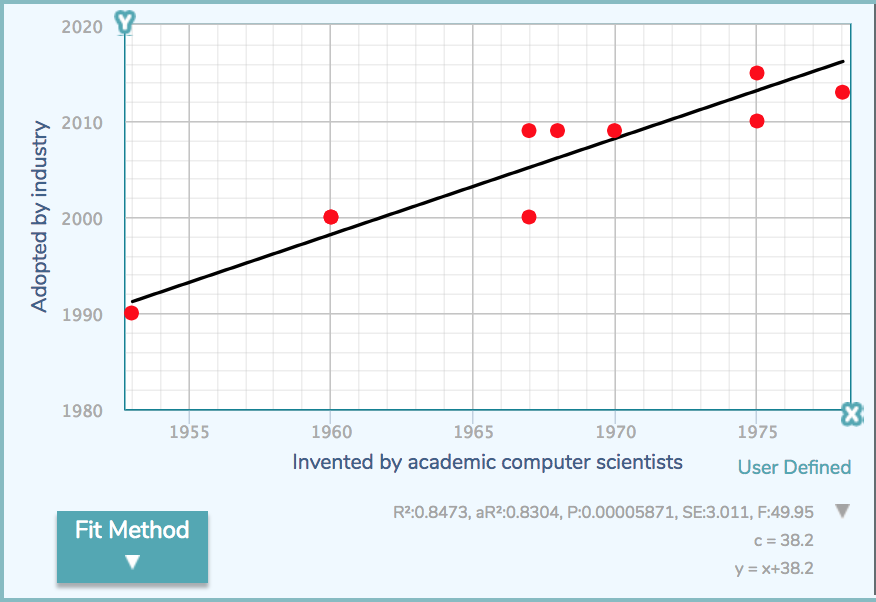
\includegraphics[width=0.7\textwidth]{40-year-gap}
\par\end{center}

\end{frame}

\begin{frame}{Current features of \texttt{Chymyst}}

\begin{itemize}
\item Blocking molecules with timeouts and back-signalling
\item Automatic pipelining of molecules (ordered mailboxes)
\item ``Static'' molecules with read-only access (similar to Akka ``agents'')
\item Compile-time and early run-time DSL error reporting
\item Logging, debugging, unit-testing facilities
\item Thread pools with thread priority control
\end{itemize}
\end{frame}

\begin{frame}{Related frameworks: Petri nets}

Workflow management: an approach based on \href{https://en.wikipedia.org/wiki/Petri_net}{Petri nets}
\begin{itemize}
\item \href{https://github.com/ing-bank/baker}{ING Baker} -- a DSL for
workflow management
\item Process modeling and control (``elevator system'' etc.)
\item Business process management (BPM) systems
\end{itemize}
\texttt{Chymyst} implements a rich version of Petri nets:
\begin{itemize}
\item Transitions admit arbitrary guard conditions and error recovery
\item Transitions carry values, reactions are values, can be nested
\item Nondeterministic, asynchronous, parallel execution
\end{itemize}
A Petri net model is straightforwardly translated into a CM program
\end{frame}

\begin{frame}{Distributed Chemical Machine}


\framesubtitle{Run concurrent code on a cluster with no code changes}
\begin{itemize}
\item \vspace{-0.2cm}
Declare some molecules as ``distributed'', of type \texttt{\textcolor{blue}{\scriptsize{}DM{[}T{]}}}{\scriptsize\par}
\item No other new language constructions are necessary!
\begin{itemize}
\item early prototype in progress, as extension of \texttt{Chymyst}
\end{itemize}
\end{itemize}
Distributed map/reduce in 15 LOC:
\begin{lyxcode}
\textcolor{blue}{\scriptsize{}implicit~val~cluster~=~ClusterConfig(???)}{\scriptsize\par}

\textcolor{blue}{\scriptsize{}val~c~=~dm{[}Int{]}~;~val~d~=~dm{[}Int{]}}\textcolor{gray}{\scriptsize{}~//~distributed}{\scriptsize\par}

\textcolor{blue}{\scriptsize{}val~res~=~m{[}(Int,~List{[}Int{]}){]}~}\textcolor{gray}{\scriptsize{}//~local}{\scriptsize\par}

\textcolor{blue}{\scriptsize{}val~fetch~=~b{[}Unit,~List{[}Int{]}{]}}{\scriptsize\par}

\textcolor{blue}{\scriptsize{}site(}{\scriptsize\par}

\textcolor{blue}{\scriptsize{}~~go~\{~case~c(x)~$\Rightarrow$~d(x~{*}~2)~\},}\textcolor{gray}{\scriptsize{}~~//~``map''~on~cluster,}\textcolor{blue}{\scriptsize{}~}{\scriptsize\par}

\textcolor{blue}{\scriptsize{}~}\textcolor{gray}{\scriptsize{}//~``reduce''~on~the~driver~node~only.}{\scriptsize\par}

\textcolor{blue}{\scriptsize{}~~go~\{~case~res((n,~list))~+~d(x)~$\Rightarrow$~res((n-1,~s::list))~\},}{\scriptsize\par}

\textcolor{blue}{\scriptsize{}~}\textcolor{gray}{\scriptsize{}//~fetch~results}{\scriptsize\par}

\textcolor{blue}{\scriptsize{}~~go~\{~case~fetch(\_,~reply)~+~res((0,~list))~$\Rightarrow$~reply(list)~\}}{\scriptsize\par}

\textcolor{blue}{\scriptsize{})}{\scriptsize\par}

\textcolor{blue}{\scriptsize{}if~(isDriver)~\{}\textcolor{gray}{\scriptsize{}~//~`true`~only~on~the~driver~node.}{\scriptsize\par}

\textcolor{blue}{\scriptsize{}~~Seq(1,~2,~3).foreach(x~$\Rightarrow$~c(x))}{\scriptsize\par}

\textcolor{blue}{\scriptsize{}~~res((3,~Nil))~;~fetch()}\textcolor{gray}{\scriptsize{}~//~Returns~the~result.}{\scriptsize\par}

\textcolor{blue}{\scriptsize{}\}}{\scriptsize\par}
\end{lyxcode}
Comparison: \href{https://github.com/ltronky/MapReduce-akka}{Akka implementation of distributed map/reduce}
(400+ LOC)
\end{frame}

\begin{frame}{Distributed cache in 10 lines of code}

\begin{itemize}
\item \vspace{-0.2cm}
Mutable \texttt{\textcolor{blue}{\scriptsize{}Map{[}String, String{]}}}
with operations: \texttt{\textcolor{blue}{\scriptsize{}put}}, \texttt{\textcolor{blue}{\scriptsize{}get}},
\texttt{\textcolor{blue}{\scriptsize{}delete}}{\scriptsize\par}
\end{itemize}
\begin{lyxcode}
\textcolor{blue}{\scriptsize{}implicit~val~cluster~=~ClusterConfig(???)}{\scriptsize\par}

\textcolor{blue}{\scriptsize{}val~data~=~dm{[}mutable.Map{[}String,~String{]}{]}}{\scriptsize\par}

\textcolor{blue}{\scriptsize{}val~put~=~dm{[}(String,~String){]}}{\scriptsize\par}

\textcolor{blue}{\scriptsize{}val~get~=~dm{[}(String,~M{[}Option{[}String{]}{]}{]}}{\scriptsize\par}

\textcolor{blue}{\scriptsize{}val~delete~=~dm{[}String{]}}{\scriptsize\par}

\textcolor{blue}{\scriptsize{}site(}{\scriptsize\par}

\textcolor{blue}{\scriptsize{}~go~\{~case~data(dict)~+~put((k,~v))~$\Rightarrow$~data(dict.updated(k,~v))~\},}{\scriptsize\par}

\textcolor{blue}{\scriptsize{}~go~\{~case~data(dict)~+~get((k,~r))~$\Rightarrow$~data(dict);~r(dict.get(k))~\},}{\scriptsize\par}

\textcolor{blue}{\scriptsize{}~go~\{~case~data(dict)~+~delete(k)~$\Rightarrow$~dict.remove(k);~data(dict)~\}}{\scriptsize\par}

\textcolor{blue}{\scriptsize{})}{\scriptsize\par}

\textcolor{blue}{\scriptsize{}if~(isDriver)~data(mutable.Map{[}String,~String{]}())}{\scriptsize\par}
\end{lyxcode}
\begin{itemize}
\item Comparison: \href{https://medium.com/@hussachai/creating-a-distributed-cache-in-100-lines-with-akka-5387bd7310fd}{Distributed cache in 100 lines of Akka}
\end{itemize}
\end{frame}

\begin{frame}{Distributed peer-to-peer chat in 15 LOC}

\begin{itemize}
\item \vspace{-0.2cm}
Register user names in chat room
\item Fetch list of users
\item Send and receive text messages
\end{itemize}
\begin{lyxcode}
\textcolor{blue}{\scriptsize{}implicit~val~cluster~=~ClusterConfig(???)}{\scriptsize\par}

\textcolor{blue}{\scriptsize{}val~users~=~dm{[}List{[}DM{[}String{]}{]}{]}}\textcolor{gray}{\scriptsize{}~//~List~of~users'~message~emitters.}{\scriptsize\par}

\textcolor{blue}{\scriptsize{}val~carrier~=~dm{[}DM{[}String{]}{]}}\textcolor{gray}{\scriptsize{}~//~Carries~this~node's~message~emitter.}{\scriptsize\par}

\textcolor{blue}{\scriptsize{}val~fetch~=~b{[}Unit,~List{[}DM{[}String{]}{]}{]}}{\scriptsize\par}

\textcolor{blue}{\scriptsize{}site(go~\{~case~users(es)~+~carrier(e)~$\Rightarrow$~users(e~::~es)~\}}{\scriptsize\par}

\textcolor{blue}{\scriptsize{},~go~\{~case~users(es)~+~fetch(\_,~r)~$\Rightarrow$~r(es)~\}~)}{\scriptsize\par}

\textcolor{blue}{\scriptsize{}~~}{\scriptsize\par}

\textcolor{blue}{\scriptsize{}val~peerName~=~???}\textcolor{gray}{\scriptsize{}~//~Read~from~config~on~node.}{\scriptsize\par}

\textcolor{blue}{\scriptsize{}val~sender~=~new~DM{[}String{]}(peerName)~}\textcolor{gray}{\scriptsize{}//~Assign~unique~molecule~name.}{\scriptsize\par}

\textcolor{blue}{\scriptsize{}site(go~\{~case~sender(x)~\ensuremath{\Rightarrow}~println(s\textquotedbl Peer~\$peerName~reads~\$x\textquotedbl )\})}{\scriptsize\par}

\textcolor{blue}{\scriptsize{}~~~}{\scriptsize\par}

\textcolor{blue}{\scriptsize{}carrier(sender)}{\scriptsize\par}

\textcolor{blue}{\scriptsize{}if~(isDriver)~users(Nil)}{\scriptsize\par}

\textcolor{gray}{\scriptsize{}//~Fetch~list~of~users~and~send~a~message~to~Sergei~if~present.}{\scriptsize\par}

\textcolor{blue}{\scriptsize{}fetch()}{\scriptsize\par}

\textcolor{blue}{\scriptsize{}~~.find(\_.name~==~\textquotedbl Sergei\textquotedbl )}{\scriptsize\par}

\textcolor{blue}{\scriptsize{}~~.foreach(sender~$\Rightarrow$~sender(\textquotedbl hello\textquotedbl ))}{\scriptsize\par}
\end{lyxcode}
\begin{itemize}
\item Comparison: \href{https://github.com/typesafehub/activator-akka-clustering/tree/master/src/main/scala/chat}{Distributed chat in > 100 lines of Akka}
\end{itemize}
\end{frame}

\begin{frame}{Reasoning in the Distributed Chemical Machine}

Distributed computing is made declarative
\begin{itemize}
\item Determine which data needs to be distributed and/or concurrent
\item Determine which computations will need to consume that data
\item Emit initial molecules and let the DCM run
\end{itemize}
Pure peer-to-peer architecture
\begin{itemize}
\item Distributed molecules may be consumed by \emph{any} DCM peer
\item All DCM peers operate in the same way (no master/worker)
\item All DCM peers need to define the same distributed reaction sites
\begin{itemize}
\item To designate a DCM peer as a ``driver'', use config files
\end{itemize}
\end{itemize}
Examples (see documentation)
\begin{itemize}
\item Broadcast (DCM peers see it exactly once upon connecting)
\item Distributed peer-to-peer chat
\end{itemize}
\end{frame}

\begin{frame}{Chemical Machine: implementation details}

\begin{itemize}
\item Each reaction site has a scheduler thread and a worker thread pool
\item Each molecule is ``bound'' to a unique reaction site
\item Each emitted molecule is stored in a multi-set at its reaction site
\item Each emitted molecule triggers a search for possible reactions
\begin{itemize}
\item Reaction search proceeds concurrently for different reaction sites
\end{itemize}
\item Reactions are scheduled on the worker thread pool
\begin{itemize}
\item The thread pool can be configured per-reaction or per-site
\end{itemize}
\item Scala macros are used for static analysis and optimizations
\begin{itemize}
\item Automatically pipelined molecules
\item Simplify and analyze Boolean conditions
\end{itemize}
\item Error analysis is also performed at early run time
\begin{itemize}
\item Reaction site with errors remain inactive
\end{itemize}
\end{itemize}
\end{frame}

\begin{frame}{Distributed Chemical Machine: implementation details}

\begin{itemize}
\item Each distributed molecule (DM) is bound to a unique reaction site
\item Emitted DM data goes into the ZK instance
\item Each DCM peer listens to ZK messages and checks for its DMs
\begin{itemize}
\item Once a DM is found, its data is downloaded and deserialized
\end{itemize}
\item On a DCM peer, each DM is identified with a unique local RS
\begin{itemize}
\item Downloaded molecules are emitted into the local RS to run reactions
\item All DCM peers must run identical reaction code for DMs
\end{itemize}
\item Each DCM peer acquires a distributed lock on its DMs
\begin{itemize}
\item Lock is released once reaction scheduling is complete
\end{itemize}
\item If a node goes down or network fails, molecules will be \emph{unconsumed}
\begin{itemize}
\item Another DCM peer will pick up these molecules later
\end{itemize}
\end{itemize}
\end{frame}

\begin{frame}{Conclusions and outlook}

\begin{itemize}
\item Chemical Machine = declarative, purely functional concurrency
\begin{itemize}
\item Similar to ``Actors'', but easier to use and ``more purely functional''
\item Significantly shorter code, easier to reason about
\end{itemize}
\item An open-source Scala implementation: \texttt{\href{https://github.com/Chymyst/chymyst-core}{Chymyst}}
\begin{itemize}
\item Static DSL code analysis (with Scala macros)
\item Industry-strength features (thread priority control, pipelining, fault
tolerance, unit testing and debugging APIs)
\item Extensive documentation: \href{https://winitzki.gitbooks.io/concurrency-in-reactions-declarative-multicore-in/content/}{tutorial book}
\end{itemize}
\item Promising applications:
\begin{itemize}
\item Workflow management
\item Distributed peer-to-peer systems
\item Process modeling, GUIs, BPM
\end{itemize}
\item Distributed Chemical Machine in the works
\end{itemize}
\end{frame}

\end{document}
peer-to-peer systems
\item Process modeling, GUIs, BPM
\end{itemize}
\item Distributed Chemical Machine in the works
\end{itemize}
\end{frame}

\end{document}
